\chapter{Cloud}\label{chap:cloud}

In this chapter we consider trade-offs stakeholders face in cloud scenarios.
Traditionally, a cloud is a set of compute and network resources, which can be elastically rented by customers.
In recent time, it has become usefull to refer to this type of cloud as \emph{machine cloud}, in order to better differentiate from the \emph{human cloud}.
The human cloud provides properties from the machine cloud, e.g. elasticity and reliability, to the crowdsourcing market by enabling employers to offer tasks to workers available on demand.
In this chapter we consider multiple scenarios:
First, we study the role of a cloud operator providing virtual resources to customers.
Then, we consider decissions faced by the a user of a cloud who is deploying virtualised network functions in a cloud.
Finally, we investigate resource dimensioning in human clouds.
Regardless of the specific scenario, the number of resoures available impact the \glspl{KPI} of all participating stakeholders, and is thus subject to optimisation.

\begin{figure}
  \centering
  \includegraphics{cloud/figures/model}
  \caption{Stakeholders investigated in the cloud scenarios}
  \label{fig:cloud:model}
\end{figure}

Thus, we first provide an overview of the involved stakeholders and \glspl{KPI} in \reffig{fig:cloud:model}.
If we study the operation of a machine cloud, both the cloud operator and the cloud user need to be considered.
The cloud operator is interested in increasing revenue, i.e. attracting a high number of customers, and decrease financial expendiature, e.g. by reducing consumed energy.
The customer of a cloud operator is interested in good \glspl{SLA}, for example a low delay before processing of a job can begin.
In the second scenario, the network function operator taking the role of a customer in the previous scenario, is interrested in provisioning a minimal number of resources from the cloud operator, in order to reduce cost, while in turn providing a sufficient \gls{SLA} to its customers.
The users of the virtualised network functions demand a sufficient availability of the provided service.
Finally, in case of the human cloud scenario, the cloud operator has to satisfy two stalkeholders with conflicting interests.
On the one hand, employers are interrested in a fast completion of the offered tasks.
On the other hand, workers are interrested in obtaining a high income.
These goals are clearly conflicting, as fast completion can be obtained by providing a high number of available workers.
However, income per workers increases if the tasks are distributed between fewer workers.
Thus, the human cloud operator has to balance the interests of the two stakeholders.

The contribution of this chapter is threefold
\begin{enumerate}
\item First, we provide a model for energy efficient data center operation and discuss sensible parameter configurations. 
\item Then, we study algorithms for resource provisioning on the example of a virtualised network function and evaluate their performance.
\item Finally, we model a crowdsourcing platform and provide guidelines for platform operators regarding resource aquisition.
\end{enumerate}

The content of this chapter is published in~\cite{Schwartz2012a,Metzger2014a,Schwartz2015}.
In \refsec{sec:cloud:related_work} we provide an overview of related work relevant to this chapter.
Then, in \refsec{sec:cloud:data_centers} we discuss the trade-offs faced by a cloud operator.
We focus on the customer of a cloud operator in \refsec{sec:cloud:virtualized_network_functions} and discuss challenges when provisioning virtualised network functions.
Strategies for resource provisioning of a human cloud are considered in \refsec{sec:cloud:crowdsourcing}.
Finally, we provide lessons learned from our studies in \refsec{sec:cloud:lessons_learned}.

\section{Background and Related Work}\label{sec:network:background}

\subsection{\headershortacr{UMTS} Networks and the \headershortacr{RRC} Protocol}\label{sec:network:background:umts_rrc}
A \gls{3G} \gls{UMTS} mobile network consists of three main components, which are depicted in \reffig{fig:network:background:mobile_network_overview}: The \gls{UE}, the \gls{RAN}, and the \gls{CN}.
The \gls{RAN} is used to establish connectivity between the \gls{UE} and the \gls{CN}, which in turn can establish connectivity to the Internet, if required.

\begin{figure}
	\centering
	\includegraphics{network/background/figures/mobile_network_overview}
	\caption{Overview of Mobile Network}
	\label{fig:network:background:mobile_network_overview}
\end{figure}

\gls{UE} consists of devices used by end users, i.e. smartphones, tablets or data card enabled notebooks, but can also include \gls{M2M} devices.
The \gls{RAN} is, amongst other tasks, responsible for \gls{RRC}, packet scheduling and handover control.
It includes network entities such as the \gls{NodeB} and the \gls{RNC}.
The \gls{CN} provides the backbone network of the \gls{UMTS} network and provides connectivity to the Internet and the \gls{PSTN}.
Furthermore, functionality such as billing, authentication and location management is provided by the \gls{CN}.

In UMTS networks, the radio resources in the RAN between base station and UE are controlled and managed by the \gls{RRC} protocol~\cite{3GPP_RRC_Spec}.
The protocol offers services such as broadcast of network information, maintenance of a connection between the \gls{UE} and \gls{RAN}, establishment of point-to-point radio bearers for data transmission, \gls{QoS} control, and reporting and cell selection management.
The protocol is divided into different parts: services for upper layers, communication with lower layers, protocol states, \gls{RRC} procedures, and error control.
In particular, \gls{RRC} also participates in the co-ordination of other resource management operations such as channel measurements and handovers.
All \gls{RRC} procedures rely on protocol states which are defined to trigger action should be applied and which information must be signaled. 
The state are defined per \gls{UE} and for the connection between the \gls{UE} and the \gls{NodeB} station.
Typically there are five \gls{RRC} states characterizing a connection between \gls{UE} and \gls{NodeB}: \gls{idle}, \gls{URAPCH}, \gls{CELLPCH}, \gls{DCH}, and \gls{FACH}.
Whether a specific \gls{RRC} state is used in a specific mobile network depends on the configuration of the network by the provider.
In the following we concentrate on the most commonly observed~\cite{Qian2010} \gls{RRC} states \gls{idle}, \gls{DCH}, and \gls{FACH}.

\subsection{Measurements of \headershortacr{RRC} Parameters and Optimisation of Resource Consumption}\label{sec:network:background:measurement_optimisation}

\subsection{Smartphone Energy Consumption and \headershortacr{QoE}}\label{sec:network:background:energy_consumption_qoe}

\section{Data Centers}\label{sec:cloud:data_centers}
\cite{Schwartz2012a}
\subsection{Problem Formulation}\label{sec:cloud:data_centers:problem_formulation}

A widely used data center architecture is the three-tier architecture shown in \reffig{fig:cloud:data_centers:problem_formulation:3-tier_datacenter}.
The upper two layers of the architecture are responsible for distributing the traffic and consist of layer 3 switches where each switch has a backup switch.
In this paper, we focus on the edge layer and here on a single \gls{POD}.
A \gls{POD} consists of a number of servers connected over top of rack switches to an aggregation switch.

\begin{figure}
  \centering
  \includegraphics{cloud/data_centers/problem_formulation/figures/architecture}
  \caption{Three-tier data center architecture}
  \label{fig:cloud:data_centers:problem_formulation:3-tier_datacenter}
\end{figure}


We assume, that new jobs entering the system arrive with exponentially distributed inter-arrival time.
When a job in form of a packet arrives at the \gls{POD}, it is forwarded to an idle server.
If no idle server is available, the job is queued.
Once a server finishes processing its current job, it picks another one from the queue.

Our goal is now to evaluate how much power is consumed in a data center and how much can be saved when servers, not processing any job, are switched off.
Therefore, we developed two different data center models.
The first model, the \emph{default data center}, consists of two-state servers only which are either \emph{busy} or \emph{idle}, as shown in \reffig{fig:cloud:data_centers:problem_formulation:servers:idle_busy}) 
For the second model, a more \emph{energy-efficient data center}, a subset of the servers may additionally be switched on and \emph{off} on demand, shown in \reffig{fig:cloud:data_centers:problem_formulation:idle_busy_off} as recommended in~\cite{EPA2007}.

\begin{figure}
	\begin{subfigure}[b]{\textwidth}
	\centering
	\includegraphics{cloud/data_centers/problem_formulation/figures/idle_busy}
	\caption{2-state server model}\label{fig:cloud:data_centers:problem_formulation:servers:idle_busy}
	\end{subfigure} 
	\begin{subfigure}[b]{\textwidth}
	\centering
	\includegraphics{cloud/data_centers/problem_formulation/figures/idle_busy_off}
	\caption{3-state model of a reserved server}\label{fig:cloud:data_centers:problem_formulation:idle_busy_off}
	\end{subfigure}

	\caption{Power state transition on a per server level}\label{fig:cloud:data_centers:problem_formulation:servers}
\end{figure}

\subsection{Default Data Center}\label{sec:cloud:data_centers:problem_formulation:default_data_center}
For the default data center model, each of the \(n\) servers is either on and processing a job or on and idle as depicted in \reffig{fig:cloud:data_centers:problem_formulation:servers:idle_busy}.
If a busy server finishes processing a job and the queue is empty, the server becomes idle. Once a new job is assigned to a yet idle server, the server becomes busy.
According to our measurements of a server with an Intel twelve core processor \SI{2.67}{\giga\hertz} and \SI{32}{\giga\byte} RAM, a server currently processing a job consumes \(e_{\text{busy}} = \SI{240}{\watt}\)
An idle server still consumes \(e_{\text{idle}} = \SI{170}{\watt}\).

\subsection{Energy-Efficient Data Center}\label{sec:cloud:data_centers:problem_formulation:energy_efficient_data_center}
For the second model, we differentiate between two types of servers.
\(n\) base-line servers which are always on and \(m\) reserved servers to be enabled on demand.
If they are enabled, their power consumption is similar to that of the default data center model.
If they are disabled, each server consumes \(e_\text{off} = \SI{0}{\watt}\).
The \(n\) servers which are always enabled consume the same power as in the default data center model.
If the system queue has a length exceeding \(\theta_2\) where \(\theta_2 \in (0, m)\) holds, the \(m\) reserved servers are enabled and stay enabled until the total number of jobs in the system drops to \(\theta_1\) for \(\theta_1 \in (0, n)\).
The transition between power levels for each of the reserved servers is depicted in \reffig{fig:cloud:data_centers:problem_formulation:idle_busy_off}.

The energy-efficient data center operation model with the parameters \(\theta_1\) and \(\theta_2\) is depicted in \reffig{fig:cloud:data_centers:problem_formulation:model} and described in detail in the next section.

\begin{figure}
  \centering
  \includegraphics{cloud/data_centers/problem_formulation/figures/model}
  \caption{System model for an energy-efficient operation}
  \label{fig:cloud:data_centers:problem_formulation:model}
\end{figure}
\subsection{Modeling}\label{sec:cloud:data_centers:modeling}
\subsubsection*{Default Data Center}\label{sec:cloud:data_centers:modeling:default}
\subsubsection*{Energy Efficient Data Center}\label{sec:cloud:data_centers:modeling:energy_efficient}
\subsection{Closed Form Solution}\label{sec:cloud:data_centers:closed_form_solution}
\subsection{Performance Evaluation}\label{sec:cloud:data_centers:performance_evaluation}

\section{Virtualised Network Functions}\label{sec:cloud:virtualized_network_functions}
\newcommand{\blockingprobability}[0]{p_B}
\newcommand{\maxServers}[0]{S_{\max}}
In this section we apply the theoretical methods discussed in \refsec{sec:cloud:data_centers} and apply them to the real-world challenge of virtualised network functions.
We consider the exemplary use case of a virtualised \gls{GGSN}.
Here, network operators consider the virtualisation of previously physical middleboxes, in order to gain elasticity and reduce costs.

In contrast to the last section, we assume a loss model, as connection establishment requests are not queued in reality but expire if no capacity is available.
Thus, we consider the blocking probability instead of the mean waiting time as a metric.
As a second metric we consider the number of provisioned servers which need to kept powered on. 

This section is structured as follows:
In \refsec{sec:cloud:virtualized_network_functions:model} we first introduce a model for a traditional \gls{GGSN}.
Then, we extend it to be applicable for the study of a virtualised \gls{GGSN}.
In \refsec{sec:cloud:virtualized_network_functions:measurement_data} we describe the procedures used to obtain and process input parameters for use in our simulation study.
Finally, in \refsec{sec:cloud:virtualized_network_functions:performance_evaluation} we study possible gains by a virtualised \gls{GGSN} by considering the tradeoff between the required servers to be active simultaneously and the incurred blocking probability. 

\subsection{Model}\label{sec:cloud:virtualized_network_functions:model}

In this section we provide a model for a traditional \gls{GGSN} and discuss a model for a virtual \gls{GGSN} using \gls{NFV}.
In \gls{NFV} \cite{Nfv2013} static network middleboxes are replaced by commodity hardware.
The tasks solved by the original middleboxes are then solved by dedicated software.

\subsubsection*{Traditional GGSN}\label{sec:cloud:virtualized_network_functions:model:traditional_ggsn}
First, we give a model for a \emph{traditional} \gls{GGSN}, i.e. a static network component.
While we consider the \gls{GGSN} to be one fixed entity, it can in reality consist of multiple servers.
However, due to the fact that the \gls{GGSN} is purchased from a vendor as a middlebox, idle servers can be neither deactivated nor reused for other purposes.

\begin{figure}
  \centering
  \includegraphics{cloud/virtualized_network_functions/model/figures/traditional_ggsn}
  \caption{Considered model of a traditional \headershortacr{GGSN}.}
  \label{sec:cloud:virtualized_network_functions:model:traditional_ggsn:model}
\end{figure}

We give present an abstract queueing model for the traditional \gls{GGSN} in \reffig{sec:cloud:virtualized_network_functions:model:traditional_ggsn:model}.
New tunnels requests arrive according to a Poisson distribution with a rate of \(\lambda(t)\) at the \gls{GGSN}.
This server will support a maximum tunnel capacity of \(c_c\).
When this capacity is reached, blocking will occur and newly incoming tunnels requests are rejected.
Traditionally, \glspl{GGSN} can be expected to be overdimensioned in such a way that this rarely happens.
If the new tunnel is accepted, it will occupy one of the serving units of the server for the duration \(\mu(t)\) of the tunnel.
As stated earlier, we can not model the tunnel duration to be markovian, resulting in a  \(M/G/c_c\) loss system.
In order to give quality of service guarantees the network operator is interested in the system's blocking probability \(\blockingprobability\), which we consider to be a key metric of our model.
Additionally, the previously described diurnal patterns can are also be modelled by adjusting the arrival and serving process distributions for each time of day.
This alternatively also allows just to investigate the busy hour and thus the system's peak load.

\subsubsection*{\headershortacr{GGSN} using Network Function Virtualisation}\label{sec:cloud:virtualized_network_functions:model:virtual_ggsn}
Next, we introduce concepts from \gls{NFV}, i.e. the idea to replace middleboxes with commodity hardware as an extended model in \reffig{sec:cloud:virtualized_network_functions:model:virtual_ggsn:model}. 
This allows us to realise benefits from cloud computing, as we are now able to scale out, instead of up.
The assumptions of the Markov arrival process \(\lambda(t)\) and the serving time distributions \(\mu(t)\) are carried over.
However, instead of one server processing every tunnel, this model assumes that there are up to \(s_{max}\) virtualised servers \(s_i\).
Each of these is less powerful than the traditional \gls{GGSN}, having a tunnel serving capacity of \(c_i \ll c_c\) and a total system capacity of \(c_{max} = s_{max} \times i\).

\begin{figure}
  \centering
  \includegraphics{cloud/virtualized_network_functions/model/figures/virtual_ggsn}
  \caption{Considered model of a virtualised \headershortacr{GGSN}.}
  \label{sec:cloud:virtualized_network_functions:model:virtual_ggsn:model}
\end{figure} 

In its initial state, for efficiency, all but a small portion of the server instances are considered to be disabled.
Only, when a certain condition is reached, a new server instance is provisioned.
As a simple example, one instance could be kept in reserve for upcoming requests and an additional would be provisioned as soon as the reserve is used.
Similar rules should apply in the shutdown of servers and form a hysteresis with the boot condition.
For example it would be possible to keep at least one server in reserve but never more than two.

If these conditions are not carefully selected and are in tune with the expected boot time of an instance, additional blocking can occur.
Despite not having reached its maximum capacity, this system would still reject tunnel requests during the provisioning phase when no tunnel slots are available.
This could be remedied by a request queue.
However, this would introduce additional complexity to the system without providing real benefit, as mobile devices or applications will repeat their attempts and would time out when the request is taking too long. 

To place incoming tunnel state on one of the available servers a load balancer is required. 
To ensure that the system in run time can scale down to its actual needs, the balancer should place tunnels on servers that are the fullest, keeping the reserve free.
It may even migrate tunnel state from almost empty servers away so that these can be shut down, when the shutdown condition is fulfilled.
Keeping instance close to their capacity should also have no impact on the performance a mobile device associated to a specific tunnel experiences.

\subsection{Mobile Network Traffic Characteristics}\label{sec:cloud:virtualized_network_functions:measurement_data}

In order to evaluate our models introduced in \refsec{sec:cloud:virtualized_network_functions:model}, we use data gathered from a nation-wide mobile operator.
This allows for precise core network evaluations and the creation statistical fits for the observed processes.
In this section we first describe the dataset used for the evaluation and afterwards, we derive the random variables required for our models.

\subsubsection*{Dataset Description}\label{sec:cloud:virtualized_network_functions:measurement_data:description}

\label{sec:dataset_description}

All data was collected by the \gls{METAWIN} monitoring system~\cite{Ricciato2006} with measurement probes located at the Gn interface within the core network, , as shown in \reffig{fig:cloud:virtualized_network_functions:measurement_data:dataset_description:mobile_network_overview}.
The Gn interface is a \gls{IP} based \gls{WAN} used to connect \gls{GGSN} and \gls{SGSN} installations.
This access to the mobile core network provides \gls{METAWIN} with a broad access to mobile signalling traffic.

\begin{figure}
  \centering
  \includegraphics{cloud/virtualized_network_functions/measurement_data/figures/mobile_network_overview}
  \caption{Overview of the \headershortacr{METAWIN} monitoring architecture in a \headershortacr{3G} mobile network~\cite{Ricciato2006}.}
  \label{fig:cloud:virtualized_network_functions:measurement_data:dataset_description:mobile_network_overview}
\end{figure}

For this investigation we employ \gls{GTP} protocol data gathered by \gls{METAWIN}.
This data includes the \gls{RAT} identifier as well as the terminal types of the mobile clients, by use of the \gls{TAC} part of the \gls{IMEI}.
To meet privacy requirements, \gls{METAWIN} anonymises all captured data.
The application-level payload is removed and all user identifiers are hashed with one-way functions before data storage.
Individual \glspl{UE} in our dataset can be differentiated by the hashed \gls{MS-ID}, but not traced back to the actual user.

The used dataset is a week-long trace from the third week of April 2011.
It consists of \(2.2\) billion aggregated flows for user traffic and \(410\) million \gls{GTP} Tunnel Management transactions.
It was tapped at one of the \glspl{GGSN} of the operator and contains about half of the total traffic volume handled by the operator in this period.

\subsubsection*{Statistical Evaluation}\label{sec:cloud:virtualized_network_functions:measurement_data:evaluation}

Using this dataset, we can obtain the distributions required for the models introduced in \refsec{sec:cloud:virtualized_network_functions:model}.
First, we study the tunnel inter-arrival time in \reffig{fig:cloud:virtualized_network_functions:measurement_data:evaluation:tunnel_iat}.

\begin{figure}
  \centering
  \includegraphics{cloud/virtualized_network_functions/measurement_data/figures/tunnel_iat}
  \caption{Empirical and exponentially fitted \headershortacrpl{CDF} of the tunnel inter-arrival duration by time of day. \headershortacrpl{CDF} are overlapping as the coefficient of determination is close to \(1\).}
  \label{fig:cloud:virtualized_network_functions:measurement_data:evaluation:tunnel_iat}
\end{figure}

The arrival of new tunnel requests can be used as a measure for the load a \gls{GGSN} experiences, as every incoming tunnel carries several signalling interactions, processing and state with it.
Typically, a device will only hold one tunnel at a time, but this tunnel can be initiated and shut down in rapid succession, causing the aforementioned issues in the radio network.
The arrivals also show a strong diurnal effect, closely resembling patterns present in the actual user traffic:
We observe a decline of arrivals, i.e. longer inter-arrivals, late in the night and during the early morning hours with a peak rate in the afternoon and early evening.
To represent this time-of-day dependence in the model, the measurement was split into the four time slots displayed in the figure.
Each slot was then fitted with an exponential distribution by way of moment matching.
This results in the cumulative negative exponential distribution function \(F(x) = 1- e^{-\lambda x}, x \geq 0\) with \(\lambda\) given in \reftab{tab:cloud:virtualized_network_functions:measurement_data:evaluation:iat_fits} for the four time slots.
The fitted functions match the empirical data, with some deviation present at the left tail but overall with a positive correlation coefficient approaching \(1\).

\begin{table}
  \centering
  \caption{Parameters for the exponentially distributed inter-arrival times and corresponding Pearson correlation coefficients.}
  \label{tab:cloud:virtualized_network_functions:measurement_data:evaluation:iat_fits}  
  \begin{tabular}{lcc}
  \toprule
  Time of day & \(\lambda\) & \(R_{arr}\)\\
  \midrule
  0h-5h & $10.67$ & $0.99$\\
  6h-11h & $24.53$ & $0.99$\\
  12h-17h & $29.25$ & $0.99$\\
  18h-23h & $23.49$ & $0.98$\\
   \bottomrule
  \end{tabular}
\end{table}

The second important tunnel property is the duration of the \gls{PDP} Context state accompanying a \gls{GTP} tunnel held at the \gls{GGSN}.
\reffig{fig:cloud:virtualized_network_functions:measurement_data:evaluation:tunnel_duration} shows the tunnel durations split up for the time of day, as there is once again a slight diurnal effect present, albeit with shifted peaks.
Longer tunnels tend to occur at night, shorter tunnels during midday.
Further properties of the tunnel duration, especially the correlation with device types and operating systems, are investigated in detail in~\cite{Metzger2014}.

\begin{figure}
  \centering
  \includegraphics{cloud/virtualized_network_functions/measurement_data/figures/tunnel_duration}
  \caption{Empirical and fitted \headershortacrpl{CDF} of the tunnel duration by time of day with fitted rational functions.}
  \label{fig:cloud:virtualized_network_functions:measurement_data:evaluation:tunnel_duration}
\end{figure}

\begin{table}
  \centering
  \caption{Inverse functions fitted to the empirical duration distribution and correlation coefficients of the fit.}
  \label{tab:cloud:virtualized_network_functions:measurement_data:evaluation:duration_fits}  
  \begin{tabular}{lcc}
  \toprule
  Time of day & Inverse fitted duration function & \(R_{dur}\)\\
  \midrule
  0h-5h & $0.91 - 60.61y - 3498.78y^3 - \frac{110.70y + 2289.94y^3}{y - 1.00}$ &  $0.99$ \\
  6h-11h & $1 + 117.48y - 368.64y^2 - \frac{1720.13y^4}{y - 1.00}$ & $0.99$ \\
  12h-17h & $0.95 + 69.49y + \frac{81146.10y^3 + 1.08\times10^6y^5}{805 - 802.01y}$ & $0.99$ \\
  18h-23h & $0.91 + 82.05y - \frac{2936.93y^4}{1.94y - 1.95}$ & $0.99$\\
  \bottomrule
  \end{tabular}
\end{table}

Furthermore, the model requires information on the tunnel durations.
However, none of the basic probability distributions, e.g. exponential, gamma, and Weibull distributions, fit the tunnel duration well enough.
One of the reasons for this probably being the correlation of the tunnel duration to a large number of factors, including user behaviour and network-specific timers and procedures, e.g. tunnels are shut down by the network after specific events, introducing artefacts which make it hard to fit any distribution against.
Instead, we fit rational functions to the empirical \gls{CDF} using the Eureqa \cite{Schmidt2009} software.

This allows for a much closer fit while still smoothing out some of the artefacts.
\reftab{tab:cloud:virtualized_network_functions:measurement_data:evaluation:duration_fits} displays these functions fitted to the inverse \gls{CDF}, to be directly used for generating random numbers using the inversion method.
Both the \gls{CDF} in \reffig{fig:cloud:virtualized_network_functions:measurement_data:evaluation:tunnel_duration} as well as the Pearson correlation coefficient confirm the goodness of the fitted functions.

\subsection{Inferring State Transitions and Deriving Metrics}\label{sec:network:network_traces:performance_evaluation}
\gls{RRC} state transitions are triggered by the \gls{UE}’s firmware.
While solutions exist to capture RRC state transitions on specific hardware~\cite{zayas2010} they are not available for all modern smartphone platforms.
Other options to measure the required information include using costly hardware and use specific \glspl{UE}, usually not available to researchers and application developers.
This prevents the developers from evaluating the effect of their applications on the overall health
of the network.
Consequently, they can not take measures to prevent the harmful behaviour of their applications.
However, it is possible to infer the \gls{RRC} state transitions for a given packet trace if the network configuration is known.

First, we describe the setup used to capture network packet traces for arbitrary apps.
Then, we give an algorithm to infer the \gls{RRC} state transitions for a given packet trace.
Based on these state transitions, we can calculate the number of signalling messages generated
by the packet trace. 
Finally, we use the information on when which \gls{RRC} state was entered to calculate the power drain of the \gls{UE}’s radio interface.

\subsubsection*{Measurement Procedure and Setup}\label{sec:network:network_traces:performance_evaluation:measurement}
To investigate the behaviour of the application under study, we capture traffic during a typical use of the application on a \emph{Samsung Galaxy SII} smartphone.
The smartphone runs the Android operating system and is connected to the \gls{3G} network of a major German network operator.
To obtain the network packet traces we use the \texttt{tcpdump} application.
This application requires \emph{root} privileges which are obtained by rooting the device and installing the custom \emph{cyanogenmod} ROM \footnote{http://www.cyanogenmod.org}.
Once \texttt{tcpdump} is installed and running, we start the application under study and capture packet traces while the application is running.
Then, the \emph{android debugging bridge} is used to copy the traces to a workstation.
The traces contain \gls{IP} packets embedded in Linux Cooked Captures.
We require the \gls{IP} packets, thus we extracted the \gls{IP} packets which are used during the following analysis.

\subsubsection*{Inferring Network State}\label{sec:network:network_traces:performance_evaluation:inferring_network_state}
In this section we study the influence of the application traffic on \gls{RRC} state transitions and signalling messages.
Since \gls{RRC} state transitions can not be captured using commonly available tools, we introduce an algorithm to infer \gls{RRC} state transitions from \gls{IP} packet traces.
Using this algorithm we analyse the \gls{RRC} state transition frequency and signalling message load for the Two State Model and Three State Model.

Traffic below the network layer can not be measured without specific equipment which interfaces with the proprietary firmware of the \gls{UE} and is often out of reach for developers interested in assessing the impact of their applications on the network.
Based on the Two State and Three State models introduced in \refsec{sec:network:background:umts_rrc}, we process \texttt{tcpdump} captures of the application traffic.
However, it should be noted that this method is not restricted to a specific network model, but can be extended to any other network model as well.
Using these captures, we extract the timestamps when \gls{IP} packets are sent or received.
Furthermore, we require the timer values of the transition from \gls{RRC_DCH} state to \gls{RRC_FACH} state, \gls{TDCH}, and the timer for the transition between \gls{RRC_FACH} and \gls{RRC_idle} states, \gls{TFACH}.
Based on these informations \refalg{alg:network:network_traces:performance_evaluation:inferring_network_state:inference_algorithm} infers the timestamps of state transitions according to the \gls{3GPP} specification \cite{3GPP_RRC_Spec} for the Three State Model.
This algorithm can be simplified to also work for the Two State Model. 
Alternatively, a method to post process the results of the algorithm to obtain results for the Two State Model is given at the end of this section.
The algorithm first computes the inter-arrival times of all packets.
Then, each timestamp is considered.
If the \gls{UE} is currently in \gls{RRC_idle} state, a state transition to \gls{RRC_DCH} occurs at the moment the packet is sent or received.
If the inter-arrival time exceeds the \gls{TDCH} timer the \gls{UE} transitions to \gls{RRC_FACH} \gls{TDCH} seconds after the packet was sent or received.
Similarly, if the inter-arrival time exceeds both the \gls{TDCH} and \gls{TFACH} timers a state transition to \gls{RRC_idle} occurs \gls{TDCH} seconds after the state transition to \gls{RRC_FACH}.

\begin{algorithm}
  \begin{algorithmic}
    \Require{Packet arrival timestamps \emph{ts}\\
    \gls{RRC_DCH} to \gls{RRC_FACH} timer \gls{TDCH}\\
    \gls{RRC_FACH} to \gls{RRC_idle} timer \gls{TFACH}}
    \Ensure{Times of state transition \emph{state\_time}\\
    New states after state transitions \emph{state}}
    \State \texttt{interarrival(i)} $\leftarrow$ \emph{ts}(i+1) - \emph{ts}(i)
    \State \texttt{index} $\leftarrow 0$
    \ForAll{ts(i)}
      \If{\texttt{state(index)} = \gls{RRC_idle}}
        \State \texttt{index} $\leftarrow$ \texttt{index} + 1
        \State \texttt{state(index)} $\leftarrow$ \gls{RRC_DCH}
        \State \texttt{state\_time(index)} $\leftarrow$ ts(i)
      \EndIf
      \If{\texttt{interarrival}(i-1) $> \gls{TDCH}$}
        \State \texttt{index} $\leftarrow$ \texttt{index} + 1
        \State \texttt{state(index)} $\leftarrow$ \gls{RRC_FACH}
        \State \texttt{state\_time(index)} $\leftarrow$ ts(i) $+ \gls{TDCH}$
      \EndIf
      \If{\texttt{interarrival}(i-1) $> \gls{TDCH} + \gls{TFACH}$}
        \State \texttt{index} $\leftarrow$ \texttt{index} + 1
        \State \texttt{state(index)} $\leftarrow$ \gls{RRC_idle}
        \State \texttt{state\_time(index)} $\leftarrow$ ts(i) $+ \gls{TDCH} + \gls{TFACH}$
      \EndIf
    \EndFor
  \end{algorithmic}
  \caption{Inferring \headershortacr{RRC} state transitions based on \headershortacr{IP} timestamps}
  \label{alg:network:network_traces:performance_evaluation:inferring_network_state:inference_algorithm}
\end{algorithm}

\gls{UE} vendors always search for ways to decrease power drain of their devices.
A straightforward way to achieve this, if only the wellbeing of the \gls{UE} is considered, is to transition from \gls{RRC_DCH} state to \gls{RRC_idle} as soon as no additional data is ready for sending.
While this transition is not directly available in the 3GPP specification for the \gls{RRC} protocol \cite{3GPP_RRC_Spec}, a \gls{UE} may reset the connection, effectively transitioning from any state to \gls{RRC_idle}.
This behaviour can be modelled using the Two State Model introduced in \refsec{sec:network:background:umts_rrc}.

State transitions for the Two State Model can be calculated using a similar algorithm.
Alternatively, the behaviour of the Two State Model can be emulated using \refalg{alg:network:network_traces:performance_evaluation:inferring_network_state:inference_algorithm} if \gls{TFACH} is set to \SI{0}{\second} and all state transitions to \gls{RRC_FACH} are removed in a post processing step.

\subsubsection*{Calculating Signalling Frequency and Power Consumption}\label{sec:network:network_traces:calculating_metrics}

\begin{table}
\centering
  \caption{Number of signalling messages per \headershortacr{RRC} state transition perceived at the \headershortacr{RNC} (Taken From \cite{3GPP_RRC_Spec})}
  \label{tab:network:network_traces:calculating_metrics:signalling_messages}
\begin{tabular}{cccc}
	\toprule
    from/to & \gls{RRC_idle} & \gls{RRC_FACH} & \gls{RRC_DCH}\\
    \midrule
    \gls{RRC_idle} & -- & 28 & 32\\
    \gls{RRC_FACH} & 22 & -- & 6\\
    \gls{RRC_DCH} & 25 & 5 & --\\
    \bottomrule    
	\end{tabular}
\end{table}

In reality, the number of state transitions is not the metric of most importance if network signalling is to be evaluated.
Each state transition results in a number of \gls{RRC} messages between the \gls{UE} and different network components.
For this study we consider the number of messages observed at the \gls{RNC}, which can be found in \cite{3GPP_RRC_Spec} and is summarized in \reftab{tab:network:network_traces:calculating_metrics:signalling_messages}.
It can be seen that transitions from or to the \gls{RRC_idle} state are especially expensive in terms of number of messages sent or received.
This is due to the fact that upon entering or leaving the \gls{RRC_idle} state, authentication has to be performed. 
Note that for the Two State Model only transitions from or to the \gls{RRC_idle} state occur.
This results in the fact that for the same network packet trace the number of signalling messages occurring in the Two State Model is generally higher than in the Three State Model.
To obtain the total number of signalling messages, we weight the number of state transitions with the number of messages sent per state transitions.
Then, we average the number of state transitions over the measurement duration to obtain a metric for the signalling load at the \gls{RNC}, i.e. the \gls{SF}.
The inference algorithm does not differentiate between state changes caused by upstream or downstream traffic.
State changes caused by downstream traffic usually generate some additional signalling messages, as paging is involved.
The inference algorithm can be easily enhanced to support this behaviour.
However, the results discussed in the next section would only change quantitatively.
Furthermore, the algorithm can be easily adapted to new networking models or signalling numbers.

\begin{table}
  \centering
  \caption{Power consumption of the \headershortacr{UE} radio interface depending on current \headershortacr{RRC} state (taken from \cite{Qian2011a})}
  \label{tab:network:network_traces:calculating_metrics:power_consumption}  
  \begin{tabular}{cc}
  	\toprule
    \gls{RRC} State & Power Consumption\\
    \midrule
    \gls{RRC_idle} & \SI{0}{\milli\watt}\\
    \gls{RRC_FACH} & \SI{650}{\milli\watt}\\
    \gls{RRC_DCH} & \SI{800}{\milli\watt}\\
    \bottomrule
  \end{tabular}
\end{table}

From a users point of view, the signalling message frequency is of little importantance.
The user is interested in a low power drain as this increases the battery life of the device.
To calculate the battery life, we use the time when state transitions occurred, and the information about the state the transition was to, to calculate the relative amount of time that was spent in each state.
Given the relative time spent in each state, we use \reftab{tab:network:network_traces:calculating_metrics:power_consumption}, taken from \cite{Qian2011a}, to compute the \gls{PD} of the radio interface during the measurement phase.
We focus on the power drain of the radio interface, as it is possible to measure the aggregated power drain using out of the box instrumentation techniques provided by the hardware vendor.
\section{Crowdsourcing Platforms}\label{sec:cloud:crowdsourcing}

\newcommand{\campaignIAT}{\ensuremath{t_c}\xspace}
\newcommand{\campaignSize}{\ensuremath{\Theta}\xspace}
\newcommand{\taskDuration}{\ensuremath{B}\xspace}
\newcommand{\meanTaskLength}{\ensuremath{E[B]}\xspace}
\newcommand{\numberOfWorkers}{\ensuremath{c}\xspace}

\newcommand{\workerUtilization}{\ensuremath{\rho}\xspace}
\newcommand{\campaignDuration}{\ensuremath{\delta}\xspace}
\newcommand{\preTaskProcessingDelay}{\ensuremath{E[D]}\xspace}

\cite{Schwartz2015}

\subsection{Model}\label{sec:cloud:virtualized_network_functions:model}

In this section we provide a model for a traditional \gls{GGSN} and discuss a model for a virtual \gls{GGSN} using \gls{NFV}.
In \gls{NFV} \cite{Nfv2013} static network middleboxes are replaced by commodity hardware.
The tasks solved by the original middleboxes are then solved by dedicated software.

\subsubsection*{Traditional GGSN}\label{sec:cloud:virtualized_network_functions:model:traditional_ggsn}
First, we give a model for a \emph{traditional} \gls{GGSN}, i.e. a static network component.
While we consider the \gls{GGSN} to be one fixed entity, it can in reality consist of multiple servers.
However, due to the fact that the \gls{GGSN} is purchased from a vendor as a middlebox, idle servers can be neither deactivated nor reused for other purposes.

\begin{figure}
  \centering
  \includegraphics{cloud/virtualized_network_functions/model/figures/traditional_ggsn}
  \caption{Considered model of a traditional \headershortacr{GGSN}.}
  \label{sec:cloud:virtualized_network_functions:model:traditional_ggsn:model}
\end{figure}

We give present an abstract queueing model for the traditional \gls{GGSN} in \reffig{sec:cloud:virtualized_network_functions:model:traditional_ggsn:model}.
New tunnels requests arrive according to a Poisson distribution with a rate of \(\lambda(t)\) at the \gls{GGSN}.
This server will support a maximum tunnel capacity of \(c_c\).
When this capacity is reached, blocking will occur and newly incoming tunnels requests are rejected.
Traditionally, \glspl{GGSN} can be expected to be overdimensioned in such a way that this rarely happens.
If the new tunnel is accepted, it will occupy one of the serving units of the server for the duration \(\mu(t)\) of the tunnel.
As stated earlier, we can not model the tunnel duration to be markovian, resulting in a  \(M/G/c_c\) loss system.
In order to give quality of service guarantees the network operator is interested in the system's blocking probability \(\blockingprobability\), which we consider to be a key metric of our model.
Additionally, the previously described diurnal patterns can are also be modelled by adjusting the arrival and serving process distributions for each time of day.
This alternatively also allows just to investigate the busy hour and thus the system's peak load.

\subsubsection*{\headershortacr{GGSN} using Network Function Virtualisation}\label{sec:cloud:virtualized_network_functions:model:virtual_ggsn}
Next, we introduce concepts from \gls{NFV}, i.e. the idea to replace middleboxes with commodity hardware as an extended model in \reffig{sec:cloud:virtualized_network_functions:model:virtual_ggsn:model}. 
This allows us to realise benefits from cloud computing, as we are now able to scale out, instead of up.
The assumptions of the Markov arrival process \(\lambda(t)\) and the serving time distributions \(\mu(t)\) are carried over.
However, instead of one server processing every tunnel, this model assumes that there are up to \(s_{max}\) virtualised servers \(s_i\).
Each of these is less powerful than the traditional \gls{GGSN}, having a tunnel serving capacity of \(c_i \ll c_c\) and a total system capacity of \(c_{max} = s_{max} \times i\).

\begin{figure}
  \centering
  \includegraphics{cloud/virtualized_network_functions/model/figures/virtual_ggsn}
  \caption{Considered model of a virtualised \headershortacr{GGSN}.}
  \label{sec:cloud:virtualized_network_functions:model:virtual_ggsn:model}
\end{figure} 

In its initial state, for efficiency, all but a small portion of the server instances are considered to be disabled.
Only, when a certain condition is reached, a new server instance is provisioned.
As a simple example, one instance could be kept in reserve for upcoming requests and an additional would be provisioned as soon as the reserve is used.
Similar rules should apply in the shutdown of servers and form a hysteresis with the boot condition.
For example it would be possible to keep at least one server in reserve but never more than two.

If these conditions are not carefully selected and are in tune with the expected boot time of an instance, additional blocking can occur.
Despite not having reached its maximum capacity, this system would still reject tunnel requests during the provisioning phase when no tunnel slots are available.
This could be remedied by a request queue.
However, this would introduce additional complexity to the system without providing real benefit, as mobile devices or applications will repeat their attempts and would time out when the request is taking too long. 

To place incoming tunnel state on one of the available servers a load balancer is required. 
To ensure that the system in run time can scale down to its actual needs, the balancer should place tunnels on servers that are the fullest, keeping the reserve free.
It may even migrate tunnel state from almost empty servers away so that these can be shut down, when the shutdown condition is fulfilled.
Keeping instance close to their capacity should also have no impact on the performance a mobile device associated to a specific tunnel experiences.

\subsection{Measurement of Platform Characteristics}\label{sec:cloud:crowdsourcing:measurements}
In this section we analyse a large dataset from a commercial crowdsourcing platform to derive to derive realistic model parameters and compare the model based on these results with the analytic approximation.

\subsubsection*{Deriving Realistic Model Parameters}
Our analysis is based on a large dataset from the commercial micro-tasking platform Microworkers.com.
The dataset contains information about more then 160.000 campaigns submitted to the platform between May 2009 and Jan 2015, including the number of task per campaign was well as the time of the submission of the campaign.  

\paragraph*{Inter-arrival Times:} First, we study the inter-arrival times of the campaigns.
During the observation period, the platform faced some downtime due to software update or changes of the technical infrastructure.
During this time, no campaigns could be submitted resulting in relatively large campaign inter-arrival times.
In our model we only consider the regular operation of the platform, therefore we removed all inter-arrival times larger then \SI{97.5}{\percent} quantile of all observed values, which affects about \SI{2.5}{\percent} of all values.

\begin{figure}
  \centering
  \includegraphics{cloud/crowdsourcing/measurements/figures/campaign_interarrival}
  \caption{Observed campaign inter-arrival times \(A_c\) and corresponding fit.}
  \label{fig:cloud:crowdsourcing:measurements:parameters:campaign_interarrival}
\end{figure}

Considering the remaining data, we observe a mean campaign inter-arrival time of \SI{0.241}{\hour} with a standard deviation \SI{0.346}{\hour}.
\reffig{fig:cloud:crowdsourcing:measurements:parameters:campaign_interarrival} shows the \gls{CDF} of considered inter-arrival times, as well as the fitted distribution.
For the fitting we considered several possible distributions but found the gamma distribution 

\[
P(A_c=t) \sim \Gamma(\alpha,\beta,t) = \frac{\beta^\alpha}{\Gamma(\alpha)} x^{\alpha-1} e^{-{\beta}t}
\]

defined by shape \(\alpha\) and rate \(\beta\) to be the most suitable.
Using \texttt{fitdistrplus}\footnote{\url{https://cran.r-project.org/web/packages/fitdistrplus}, \accessed} for the R language we derive the distribution parameters for the campaign inter-arrival times \(\campaignIAT\) by moment fitting and result in the estimated parameters \(\alpha=0.484\) and \(\beta=2.009\).

\paragraph*{Campaign Sizes:}Next, we consider the campaign sizes, respectively the number of tasks per campaign.
The smallest possible campaign sizes on Microworkers is \(30\) tasks, however our dataset contained a few internal test campaigns with a small size.

These test campaigns, as well as outliers larger than the \SI{97.5}{\percent} quantile of the campaign size have been removed from the considered dataset.
In total \SI{3.7}{\percent} of the original dataset were filtered by these conditions, the remaining data resulted in a mean campaign size of \(97.01\) tasks and a standard deviation of \(103.41\).
The \gls{CDF} of the campaign sizes \campaignSize is depicted in \reffig{fig:cloud:crowdsourcing:measurements:parameters:campaign_sizes}, together with the corresponding fitted distribution.

\begin{figure}
  \centering
  \includegraphics{cloud/crowdsourcing/measurements/figures/campaign_sizes}
  \caption{Observed campaign sizes \campaignSize and corresponding fit.}
  \label{fig:cloud:crowdsourcing:measurements:parameters:campaign_sizes}
\end{figure}

Due to the platform restrictions mentioned above, the campaign sizes start with a minimum value of \(30\) tasks.
We observer that a very high share, i.e. \SI{35}{\percent}, of campaigns has only this minimum size.
Further, campaign sizes which are a multiple of \(10\) or a multiple of \(100\) are quite frequent.
This is caused by the fact that most task on Microworkers.com are repetitive and the employers choose the required number of repetitions and thus are more likely to round the number of repetitions to the nearest multiple of \(10\) or \(100\).

In order to obtain an suitable analytic distribution for the empiric values, we normalise the observed values and use the following piecewise defined distribution.
\begin{equation*}
P(S=s) \sim
\begin{cases}
  0 & \text{if } s < s_{\min}\\
  p_{s_{\min}} & \text{if } s=s_{\min} \\
  GEOM(s) \cdot 10 + (s_{\min}+1) & \text{else}
\end{cases}
\end{equation*}
with 
\begin{equation*}
GEOM(s) = {(1-p)}^s p.
\end{equation*}
The minimum campaign size \(s_{\min}\) is observed with a fixed probability \(p_{s_{\min}}\), while all campaign sizes larger then \(s_{\min}\) follow a shifted and scaled geometric distribution.

Due to the relatively high frequencies of campaign sizes being multiples of \(10\) and \(100\), it is only possible to achieve a good fitting either for the lower or the higher region of the geometric part.
As an overestimation of the campaign size will give us an upper bound of the platform work load, we decided to put a stronger emphasis on correct fitting of the larger campaign sizes.

We estimate the \(p=0.086\) parameter of the geometric distribution using quantile matching for the \SI{90}{percent} quantile.
The values \(s_{\min}=30\) and \(p_{s_{\min}}=0.350\) are obtained from the empirical values.

\paragraph*{Task Duration: }Another relevant model parameter is the length of the tasks \taskDuration, i.e., the time a single worker needs to complete one task.
Unfortunately, this information cannot be obtained from our dataset, as tracking of the individual workers is not possible.
Therefore, we assume that the processing times follow a negative-exponential distribution, i.e.
\begin{equation*}
P(t_p=t) \sim \mu  e^{-{\mu}t}.
\end{equation*}
Even if the exact processing times are not available, each employer has to add an estimation about the time it takes to complete a task in the campaign description.
In our dataset, \SI{87.8}{\percent} of all tasks had an estimated completion time between \SIrange{60}{300}{\second}.
Therefore, we consider \(\mu \in \{\frac{1}{6},\frac{1}{5},\hdots,\frac{1}{2}\}\) for the following evaluations.

\paragraph*{Number of Workers: }Finally, the last model parameter to estimate is the number of users \numberOfWorkers on the crowdsourcing platform. 
At the time of this analysis, Microworkers.com had over 650.000 registered user accounts.
However, this number is not applicable in the proposed model, for multiple reasons.
The proposed model does not consider vacation times, i.e., the workers would have to be available 24/7.
In reality, many crowdsourcing workers only work occasionally on the platforms or only for a few tasks.
Further, employers can limit the access of to their campaigns to specific subset of all workers, which is also not considered in the model.
Moreover, Microworkers also limits the number of tasks a worker can complete in a single campaign.
Taking this into account, the number of workers to be considered in our model has to be much small then the number of workers on the real world platform and consequently we decided to estimate meaningful values based on the model parameters instead of using the given number of workers from the dataset.

\subsubsection*{Comparison of Detailed and Analytical Model}
An important question for the later analysis is whether the analytic model from \refsec{sec:cloud:crowdsourcing:model} can be used as an approximation or if a simulative evaluation is necessary.
To this end we compared the later considered metrics utilisation \workerUtilization and task pre-processing delay \preTaskProcessingDelay for 
\begin{enumerate*}
\item a simulation using the empiric distributions for the task inter-arrival times and campaign sizes,
\item a simulation using the fitted distributions derived earlier in this section, and
\item the analytic model derived in \refsec{sec:cloud:crowdsourcing:model}.
\end{enumerate*}
For the analytical model we used the campaign size distribution derived in this section and \(\lambda=\SI{4.14}{\per\hour}\).
The results of the different models are shown in \reffig{fig:cloud:crowdsourcing:measurements:comparison:distribution}.

\begin{figure*}
	\centering
	\begin{subfigure}{\columnwidth}
		\includegraphics{cloud/crowdsourcing/measurements/figures/distribution_utilization}
		\caption{Utilization \workerUtilization}
		\label{fig:cloud:crowdsourcing:measurements:comparison:distribution:utilization}
	\end{subfigure}

	\begin{subfigure}{\columnwidth}
		\includegraphics{cloud/crowdsourcing/measurements/figures/distribution_task_delay}
		\caption{Mean task pre-processing delay \preTaskProcessingDelay}
		\label{fig:cloud:crowdsourcing:measurements:comparison:distribution:task_delay}
	\end{subfigure}
	\caption{Comparison of campaign arrival distributions.}
	\label{fig:cloud:crowdsourcing:measurements:comparison:distribution}
\end{figure*}

The utilisation \workerUtilization is depicted in \reffig{fig:cloud:crowdsourcing:measurements:comparison:distribution:utilization}, the task pre-processing delay \preTaskProcessingDelay in \reffig{fig:cloud:crowdsourcing:measurements:comparison:distribution:task_delay}.
In both figures, the x-axis shows the number of workers \(\numberOfWorkers\).
The line colour indicates the mean task length, ranging from \SIrange{120}{360}{\second}, the line style denotes the underlying model.
We observe that all models result in the same utilisation \workerUtilization, which is not surprising when considering \(\workerUtilization = \frac{E[A_c] E[\campaignSize]}{c\mu}\) with the mean inter-arrival time \(E[A_c]\).
Here, all parameters are the same for the three compared models and therefore, no significant differences can be seen.

This is different for the task pre-processing delay \preTaskProcessingDelay. 
Here, large discrepancies can been observed between the model based on the empiric distributions and the analytical model.
This results show that the \(M^{[\campaignSize]}/M/\numberOfWorkers-\infty\) model can also not be used as a worst case estimations, due to the fact that it underestimates the task pre-processing delay \preTaskProcessingDelay.
In contrast to this, the simulation model based on the gamma distribution fit quite accurate the model based on the empirical values.
Therefore, we decide continue our evaluation with the simulation model, based on the gamma distributed inter-arrival times and the piecewise defined distribution for the campaign sizes.

\subsection{Numerical Evaluation}\label{sec:application:lte_video:numerical_evaluation}

In this section we study the metrics introduced in \refsec{sec:application:lte_video:system_model:model_assumptions:metrics} on the different transmission mechanisms.

First, we study the impact of the considered transmission mechanisms on the energy consumption and the wasted traffic. 
Then, in \refsec{sec:application:lte_video:connection_count} we consider the impact of the connection count for the \streaming mechanisms and varying values of the parameters \emph{stop threshold} \bufferlower and \emph{threshold size} \buffersize in more detail.

We consider a video of \(\videolength=\SI{1600}{\second}\) length which is viewed on a \gls{UE} with \gls{LTE} access.
The median of available downlink throughput in current \gls{LTE} networks is \(\bandwidth = \SI{12.74}{\mega\bit\per\second}\) \cite{Huang2012}.
A wide set of video bitrates between \SIlist{1;50}{\mega\bit\per\second} is in use~\cite{YouTube2013}.
In order to prevent stalling, we consider bitrates between \SIrange{1}{10}{\mega\bit\per\second}, staying below the available network bandwidth.
For the \streaming mechanism, a stop threshold of \(\bufferlower = \SI{4}{\second}\) and a threshold size of \(\buffersize = \SI{32}{\second}\) were selected.
Furthermore, we specify a prebuffering duration of \(\streamingstart = \SI{5}{\second}\).

We conduct our study using deterministic discrete event simulation which uses no random variables.
The wasted traffic is obtained analytically using the abort behaviour model.
Thus, all results are exact under the previously stated assumptions.

\subsubsection*{Energy Consumption}\label{sec:application:lte_video:numerical_evaluation:energy_consumption}
First, we study the influence of both video bitrate as well as the selected download mechanism on energy consumption in \reffig{fig:application:lte_video:numerical_evaluation:energy_consumption:bitrate2energy}.
\begin{figure}
  \centering
  \includegraphics{application/lte_video/numerical_evaluation/figures/bitrate2energy}
  \caption{Influence of bitrate and download mechanism on energy consumption}
  \label{fig:application:lte_video:numerical_evaluation:energy_consumption:bitrate2energy}
\end{figure}

We consider the \download mechanism and observe that it consumes the least amount of energy.
Here the video is downloaded with full bandwidth, as seen in \reffig{fig:application:lte_video:system_model:video_model}, resulting in a very short energy intensive download phase and a longer energy un-intensive playback phase.
For the \live mechanism we observe the opposite, i.e. the highest energy consumption for all bandwidths.
If this mechanism is used, the used bandwidth equals the video bitrate.
Thus, the download requires the same amount of time as the playback, resulting in the highest possible energy consumption.
The \serviceprovisioning method uses a higher bandwidth, thus reducing the overall download time.
This reduced download time decreases the energy consumption when compared to the \live mechanism, even though the bandwidth used for downloading is increased to \SI{120}{\percent}.
For the \streaming mechanism we observe an energy consumption slightly higher than the \download mechanism.
As the bitrate of the video increases, the energy consumption increases as well.
This is due to the fact that a higher video bitrates require larger downloads.
For video bitrates approaching the available bandwidth the \streaming mechanism degenerates to the \live mechanism, as no prebuffering is possible.
We conclude that the \download and \streaming mechanisms outperform \live and \serviceprovisioning with regard to energy consumption.

\subsubsection*{Wasted Traffic}\label{sec:application:lte_video:numerical_evaluation:wasted_traffic}
Next, we consider the wasted traffic as a metric of the transmission mechanism quality.
If a user completely watches a video, no traffic is wasted.
Thus, we consider only the cases where a user stops the playback before the video is finished.
\begin{figure}
  \centering
  \includegraphics{application/lte_video/numerical_evaluation/figures/bitrate2lostData}
  \caption{Influence of bitrate, download mechanism and user model on wasted traffic}
  \label{fig:application:lte_video:numerical_evaluation:energy_consumption:bitrate2lostData}
\end{figure}
In \reffig{fig:application:lte_video:numerical_evaluation:energy_consumption:bitrate2lostData} we study the wasted traffic for different video bitrates.
We consider the different transmission mechanisms introduced in \refsec{fig:application:lte_video:system_model:video_model} as well as the previously introduced user models.
We observe that the choice of user model has no significant impact on the wasted traffic.
For the \download mechanism, the amount of wasted traffic increases up to a video bitrate of \SI{6}{\mega\bit\per\second}, then the wasted traffic decreases as only video data which has been prebuffered can be lost if the user aborts the video.
As we assume a available bandwidth of \SI{12.74}{\mega\bit\per\second}, the bandwidth available for prebuffering decreases as the bitrate increases, resulting in lower amounts of wasted traffic for high video bitrates.
For the \live mechanism, we see that the wasted traffic for all user models is very low, but wasted traffic exists.
This is due to the traffic already sent by the server while the \gls{UE} is still waiting for promotion from \rrcidle to \rrcconnected, i.e. a short prebuffering phase exists.
As the bandwidth increases with the video bitrate, the wasted traffic increases as well.
Next, we consider the \serviceprovisioning approach and see an increase of wasted traffic as the video bitrate increases, due to the fact that the bandwidth used for continuous download is a factor of the video bitrate.
A higher video bitrate results in the download of the video being completed earlier, which leads to more wasted traffic.
Similar results can be seen for the \streaming mechanism, which results in more wasted traffic than the \live mechanism, but significantly less traffic than the \serviceprovisioning mechanism.
This is due to the fact that if the user aborts, at least the amount of video given by the \emph{stop threshold} \bufferlower and at most the complete buffer, given by the \emph{stop threshold} and the \emph{threshold size} are lost.
We have observed that the choice of user model results in no qualitative changes in wasted traffic.
As we have seen, the \download and \streaming mechanisms provide best results with regard to energy consumption.
However with regard to wasted traffic, the \live and \streaming mechanisms are most suited.
Thus, the \streaming mechanism seems to be a good compromise.
The network operator can select a tradeoff between energy consumption and wasted traffic as discussed in the next section.
From now on, we only consider the uniformly distributed user model.

\subsubsection*{Connection Count}\label{sec:application:lte_video:connection_count}
The \gls{ISP} is interested in reducing the number of connections occurring during video transmission.
Thus, we quantify the impact of the selected video transmission mechanism on the connection count, which directly correlates with the occurring signalling.
\begin{figure}
  \centering
  \includegraphics{application/lte_video/numerical_evaluation/figures/bitrate2connections}
  \caption{Influence of bitrate and download mechanism on connection counts}
  \label{fig:application:lte_video:numerical_evaluation:energy_consumption:bitrate2connections}
\end{figure}

In \reffig{fig:application:lte_video:numerical_evaluation:energy_consumption:bitrate2connections} we study the impact of the different transmission mechanisms on the number of connections per transmission and thus the amount of generated signalling.
We observe that for the transmission mechanisms download, live, provisioning the number of connections is constantly one, independent of the selected bitrate \bitrate.
This is due to the fact that in these transmission mechanisms the video is transmitted in one chunk.
For streaming, the number of connections decreases as the video bitrate increases.
Here, a connection occurs each time the buffer is refilled.
For larger bitrates, refilling the buffer requires a longer transmission.
As the maximum time of video transmission is upper bounded by the video length, longer buffering phases result in a smaller total amount of buffering phases and thus in less connections per video transmission.

\begin{figure}
  \centering
  \includegraphics{application/lte_video/numerical_evaluation/figures/bitrate2connections_parameters}
  \caption{Influence of bitrate and selected parameters on connection counts for the streaming mechanism}
  \label{fig:application:lte_video:numerical_evaluation:energy_consumption:bitrate2connections_parameters}
\end{figure}

Next, we consider the impact of the lower buffer threshold \bufferlower and buffer size \buffersize on the number of connections \connectioncount caused by the \streaming mechanism.
In \reffig{fig:application:lte_video:numerical_evaluation:energy_consumption:bitrate2connections_parameters} we observe that while the buffer size has a significant impact on the number of connections during a video transmission, the lower buffer threshold has almost no impact.
For buffer sizes of \SIrange{4}{8}{\second}, no signalling occurs.
This is due to the fact that, as discussed in \refsec{sec:application:lte_video:system_model:lte_network_model}, the connection timeout in \gls{UE} is configured as \SI{11.576}{\second}.
Thus, for this low buffer sizes the \gls{UE} does not disconnect from the network.
Furthermore, we observe that as the buffer size increases, the number of connections decreases.
Refilling larger buffers requires, similar to larger bitrates, longer transmission times.
Thus, due to the total upper bound on the transmission time, less download phases can occur during the transmission.
\section{Lessons Learned}\label{sec:cloud:lessons_learned}
In this chapter we examined tradeoffs between stakeholders in cloud environments.
As in the previously considered scenarios, various stakeholders exist, each with different and partially conflicting interests.
First, we considered the operation of a data centre from the point of view of a \emph{data centre operator}.
The data centre operator is interested in decreasing expenditures, e.g. due to energy consumption of computing equipment as well as in offering a competitive service to its customers.
The \emph{data centre customers} are interested in obtaining such services, usually by selecting them according to metrics specified in a \gls{SLA}.
One example of a metric considered in a \gls{SLA} is the delay a scheduled job is experiencing.
Second, we consider the role of the data centre customer in more detail.
Thus, we focus on a specific virtualised network function deployed in a data centre, and the customer in the role of a \emph{network function operator}.
The network function operator is interested in reducing the number of concurrent virtual machines provisioned, in order to decrease cost.
The network function operator in turn needs to satisfy its customers, the \emph{network function users}, who rely on the network function operator satisfying availability goals, e.g. the ability to connect to the Internet using \gls{GTP} tunnels.
Finally, we consider a human cloud scenario.
Here, the \emph{crowdsourcing platform operator} attempts to balance the needs of its two stakeholders, the \emph{crowdsourcing employer} against the requirements of the \emph{crowdsourcing worker}.
The crowdsourcing employer publishes tasks via the crowdsourcing platform to crowdsourcing employees and requires a fast task completion time.
The crowdsourcing worker is interested in being offered as many tasks as possible, in order to increase the income.
The crowdsourcing platform operator can dimension the number of available crowdsourcing workers in order balance this tradeoff. 

We draw three major conclusions from this chapter:

First, we observe that the proposed scheme for operation of the data centre allows for a reduction of the energy consumption by \SI{40}{\percent}.
As a tradeoff, the time before a task can begin processing is increased by less then \SI{1}{\milli\second}.
Furthermore, we show that for the considered mechanism, server deactivation should occur as soon as possible, resulting in the greatest energy savings while keeping an acceptable time until tasks can begin processing. 

Second, we study the existence of configurations for the virtualised network function scenario, so that even for conservative server startup times, e.g. \SI{300}{\second}, the blocking probability increases only by a factor of 1.46.
This configuration also allows  \SI{45}{\percent} of the required instances to be used for other purposes at \SI{50}{\percent} of the time. 
We also demonstrate that the observed blocking probability can be reduced by over \SI{90}{\percent} by employing techniques to reduce instance startup time, e.g. \glspl{SSD} or software containerisation.

Finally, we show that according to our model, crowdsourcing platforms are robust regarding different shapes of the arrival process, i.e. bursty arrivals compared to periodic arrivals.
Furthermore, we show that a relatively small number of workers is sufficient to sustain the platform during times of worker shortage, if the workers are put on retainer for the platform.

In the scenarios considered in this section, the platform operator is in control over parameters influencing the \glspl{KPI} for the participating stakeholders.
However, in all cases the \glspl{KPI} of the other stakeholders, by means of \gls{SLA} design, availability goals, or income, are also a \gls{KPI} for the platform operator.
This is due to the fact that not only one platform operator exists but multiple platform operators compete for customers.
Research on such multi-operator scenarios can be performed using the models introduced in this chapter.